% Method verified against the current AV + Whisper + Feature + LTX clip-Event code.
% Source map, equations, and remaining author decisions: review/方法重写与实现核对_20261108.md.
\section{Method}
\label{sec:method}

\begin{figure*}[t]
\centering
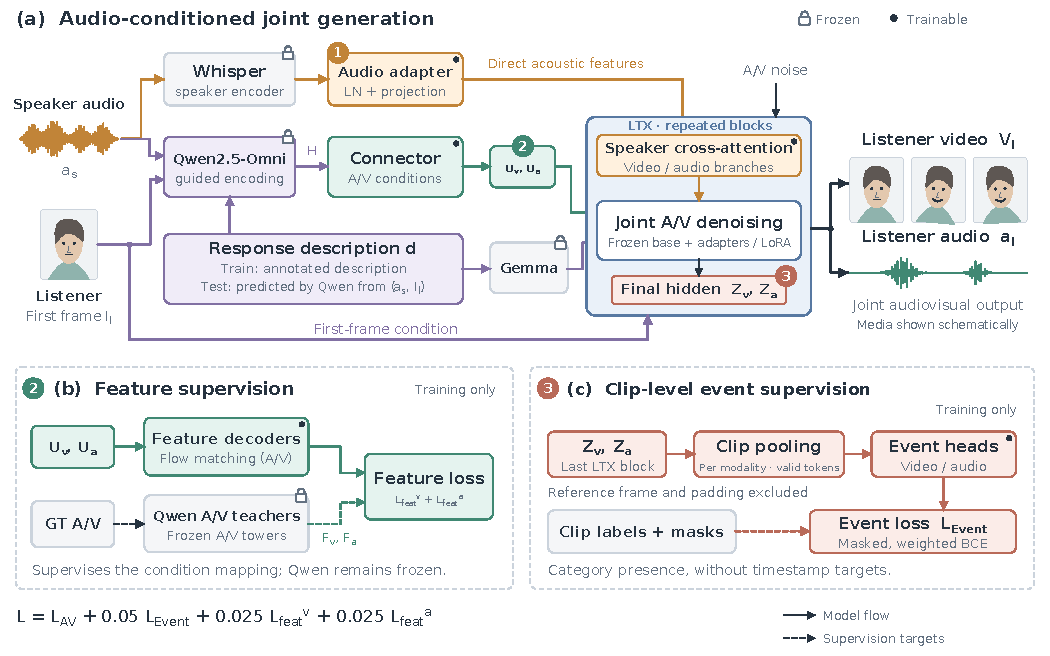
\includegraphics[width=\textwidth]{F3_method.pdf}
\caption{\figdraft{F3: Generation framework and training supervision} A connector maps guided Qwen representations to video and audio conditions, which are appended to Gemma text conditions. An independent Whisper path supplies speaker-audio features to both LTX streams. Feature supervision trains the condition mapping with frozen target-media features; clip-level Event supervision reads the final LTX block. Training uses annotated descriptions, whereas inference predicts and re-encodes descriptions from the permitted inputs. Both auxiliary objectives are used only during training. Portraits and waveforms are schematic.}
\label{fig:method}
\end{figure*}

\subsection{Overview}
\label{sec:conditioning}
\label{sec:task}
\paragraph{Task definition.}
Given the current speaker audio
$a_s$ and a listener reference
image $I_l$, we generate audiovisual
feedback as
\begin{equation}
    (\widehat V_l,\widehat a_l)
    = \mathcal{G}_{\Theta}(a_s,I_l),
    \label{eq:task}
\end{equation}
where $\mathcal{G}_{\Theta}$ denotes
the generation framework,
and $\widehat V_l$ and $\widehat
a_l$ are the listener video
and audio over the corresponding
interval.
We focus on feedback while the
speaker holds the conversational
floor, including facial expressions,
head movements, quiet
listening and brief
vocal acknowledgments.

\paragraph{Overview.}
Our framework uses a LoRA-adapted Qwen2.5-Omni
model~\cite{qwen25omni} to predict a reaction description $d$
from the speaker audio $a_s$ and listener image $I_l$.
The model then re-encodes these inputs together with $d$ to
obtain multilayer hidden states $H$, while
Gemma~\cite{gemma_pending} encodes the same description into
text conditions. A trainable connector $C_\theta$ maps $H$
into video and audio conditions:
\begin{equation}
    (U_v,U_a)=C_\theta(H),\qquad
    c_m=[G_m(d);U_m],\quad m\in\{v,a\},
    \label{eq:conditions}
\end{equation}
where $G_m(d)$ denotes the processed Gemma context for modality
$m$, and brackets denote token concatenation.

The concatenated conditions $c_v$ and $c_a$ enter the LTX
generator~\cite{ltx_pending} through its native text
cross-attention. A separate Whisper branch~\cite{whisper}
supplies direct speaker-audio features through additional
cross-attention in both generation streams. Together with
the listener reference image, these conditions guide the
joint generation of listener video and audio.

During generator training, the annotated reaction description
$d^*$ replaces the predicted description. Target audiovisual
feature supervision adapts the connector outputs $U_v$ and
$U_a$ to listener generation, while clip-level event supervision
acts on the final LTX hidden states to encourage the
corresponding feedback categories to occur.

At inference, Qwen predicts a reaction description $\hat d$
from $a_s$ and $I_l$, and then processes the original inputs
together with $\hat d$ to produce guided hidden states.
Gemma encodes the same description into text conditions.
Both conditions guide the subsequent audiovisual generation.

\subsection{Direct Speaker-Audio Conditioning}
\label{sec:direct-audio}
% Paragraph role P04: Whisper动机与设计——保留直接声学信息，补充描述与高层条件。
A reaction description summarizes intended behavior, but does not
explicitly preserve every local acoustic cue in the speaker's utterance.
We therefore provide a separate path from speaker audio to the generator.
A frozen Whisper-large-v3 encoder~\cite{whisper} extracts a
temporal feature sequence from the speaker audio. A trainable
LayerNorm and linear adapter map these features to speaker
context $S$. At each LTX block $b$, independent cross-attention
branches inject $S$ into the video and audio streams.
For modality $m\in\{v,a\}$, the attention computation within
each head is
\begin{equation}
\begin{aligned}
    Q_{b,m} &= \mathcal{P}^{Q}_{b,m}(h_{b,m}),\\
    K_{b,m} &= \mathcal{P}^{K}_{b,m}(S),\qquad
    V_{b,m} = \mathcal{P}^{V}_{b,m}(S),\\
    A_{b,m} &= \operatorname{softmax}\!\left(
        \frac{Q_{b,m}K_{b,m}^{\top}}{\sqrt{d_k}}
        +\mathcal{M}
    \right)V_{b,m},
\end{aligned}
\label{eq:speaker-attention}
\end{equation}
where $h_{b,m}$ denotes the generation hidden states,
$d_k$ is the head dimension, and $\mathcal{M}$ masks padded
speaker tokens.Queries and keys are normalized and augmented with temporal
RoPE before attention, while values are obtained by a linear
projection of the adapted speaker features $S$.

Temporal RoPE uses a common time origin in seconds for the
speaker and generation features. Leading and internal speaker
silence are retained. The multi-head attention outputs are
projected back into their respective streams and added
residually, with zero-initialized output projections.
The adapter and attention branches are optimized through
the audiovisual generation and event-supervision objectives.

\subsection{Target Audiovisual Feature Supervision}
\label{sec:feature}
% Paragraph role P06: Feature动机——让实际送入生成器的条件携带目标媒体信息。
The connector must transform general multimodal representations into
conditions useful for listener generation. To supervise this mapping,
we extract target features $F_v$ and $F_a$ from real listener video and
processed audio using frozen Qwen visual and audio encoders. 
For feature supervision, each condition token in $U_m$ is
paired with the corresponding target feature in $F_m$.
An auxiliary decoder $D_{\phi_m}$ for each modality learns
to recover target features conditioned on $U_m$, following the
AdaLN-modulated feature-decoder design of Bernini~\cite{bernini_pending}.

% Paragraph role P07: Feature公式——独立噪声下的特征流匹配，保留有效位置与安静音频。
For each valid feature position, we sample Gaussian noise $\epsilon$
and a noise level $\sigma\sim\mathcal U(0,1)$, forming
$x_{\sigma,m}=(1-\sigma)F_m+\sigma\epsilon$. The decoder predicts
the flow velocity toward noise, with objective
\begin{equation}
 \mathcal L_{\mathrm{Feature}}^m =
 \mathbb E_{\sigma,\epsilon}\!\left[
 \big\|D_{\phi_m}(x_{\sigma,m},\sigma,U_m)
       -(\epsilon-F_m)\big\|_{\Omega_m}^{2}\right].
\label{eq:feature}
\end{equation}
Here, $\Omega_m$ contains positions with valid target features
and conditioning tokens. For each sample, the error is averaged
over these positions and feature dimensions, and then averaged
across samples. Silent audio is retained as a valid target.

The auxiliary decoders and LTX share the same conditioning
representations $U_m$. Feature-loss gradients propagate through
the decoders to the connector, encouraging $U_m$ to capture
information relevant to the target listener audio and video.
The auxiliary decoders and target-feature encoders are used
only during training.

\subsection{Clip-Level Event Supervision}
\label{sec:event}
To explicitly supervise the presence of feedback categories,
we apply clip-level event supervision to the LTX generator.
The video and audio hidden states $Z_v$ and $Z_a$ from its
final Transformer block are pooled into a clip representation
for each modality. Video pooling averages spatial tokens
within each time step, followed by temporal averaging;
audio pooling averages over temporal positions.
Only valid generated positions participate in pooling,
excluding reference-frame and padding tokens.
Two modality-specific event heads then map the pooled
representations to clip-level category logits.

% Paragraph role P10: Event标签与公式——区分正例、弱负例和未知，按有效样本归一化。
Clip-level targets are extracted from reaction descriptions
using the checks described in \cref{sec:annotation}.
Each clip--category pair is assigned a positive label,
a weak negative, or an unknown status. Supported positives
receive weight 1. An unmentioned category receives
weak-negative weight 0.1 only when the description passes
the completeness checks. Uncertain or conflicting labels
are excluded from supervision.

For sample $i$ and category $c$, let $s_{ic}$ denote the
predicted logit, $y_{ic}$ the binary target, and $M_{ic}$
the validity mask. The sample weight $w_{ic}$ follows
the rules above. The event loss averages the weighted
classification error within each category and then
across valid categories:
\begin{equation}
    \mathcal L_{\mathrm{Event}}
    =
    \frac{1}{|\mathcal C_{\mathrm{eff}}|}
    \sum_{c\in\mathcal C_{\mathrm{eff}}}
    \frac{1}{N_c}
    \sum_i M_{ic}w_{ic}\,
    \mathrm{BCE}_{\alpha_c}(s_{ic},y_{ic}),
    \label{eq:event}
\end{equation}
where $N_c=\sum_i M_{ic}$ counts valid targets for category
$c$, and $\mathcal C_{\mathrm{eff}}$ contains enabled
categories with $N_c>0$. The positive-class weight
$\alpha_c$ is computed from training-label statistics
to account for class imbalance. Normalization by $N_c$
preserves the reduced contribution of weak negatives.

% Paragraph role P11: 整段监督动机——语境约束反馈方向，具体时序允许多种合理实现。
The current utterance provides cues about the affective or
attitudinal character of an appropriate response. 
%   For example, positive news may elicit smiling or shared laughter, while a
%   head shake can express disagreement. 
Even when conveying a
similar intent, listeners may react at different moments,
with different durations and repetition counts. A single
recorded response therefore represents only one plausible
temporal realization.

Motivated by this variability, our event objective supervises
the presence of feedback categories over the entire clip.
It explicitly encourages the annotated categories to occur
without prescribing their onset times, durations, or repetition
counts. This behavior-level supervision complements the
audiovisual objective, which continues to supervise the paired
listener audio and video.



\subsection{Training and Inference}
\label{sec:training}
\paragraph{Joint objective.}
% Paragraph role P12: AV目标——双路潜空间流匹配，固定参考首帧并屏蔽无效支持。
The audiovisual generator is trained with a flow-matching
objective. For each modality $m\in\{v,a\}$, a frozen VAE
encodes the target media into latents $x_0^m$. At generated
positions, Gaussian noise $\epsilon_m$ is added at a sampled
noise level $\tau$:
\begin{equation}
    x_\tau^m=(1-\tau)x_0^m+\tau\epsilon_m.
    \label{eq:av-noising}
\end{equation}

Conditioned on the inputs described above, LTX jointly
predicts video and audio velocities $\widehat v^m$,
with targets $\epsilon_m-x_0^m$. The audiovisual loss is
\begin{equation}
    \mathcal L_{\mathrm{AV}}
    =
    \mathbb E\!\left[
    \sum_{m\in\{v,a\}}
    \operatorname{MSE}_{\mathrm{valid}}
    \left(\widehat v^m,\epsilon_m-x_0^m\right)
    \right],
    \label{eq:av}
\end{equation}
where $\operatorname{MSE}_{\mathrm{valid}}$ averages the
squared error over valid generated latent positions and
feature dimensions. The reference-frame latent remains
fixed, and padding positions are excluded from the loss.



% Paragraph role P13: 总目标——Whisper是条件路径，Feature与Event是辅助监督。
The overall training objective combines audiovisual generation,
feature reconstruction, and event supervision:
\begin{equation}
\begin{aligned}
    \mathcal L ={}&
    \mathcal L_{\mathrm{AV}}
    +0.05\mathcal L_{\mathrm{Event}}\\
    &+0.025\sum_{m\in\{v,a\}}
    \mathcal L_{\mathrm{Feature}}^m.
\end{aligned}
\label{eq:total}
\end{equation}
This objective jointly optimizes the connector, Whisper
conditioning branch, LTX attention LoRA, and auxiliary
feature decoders and event heads.

\paragraph{Inference.}
Given $a_s$ and $I_l$, Qwen predicts a reaction description
$\hat d$ and processes it together with the original inputs
to obtain guided hidden states. The connector maps these
states to $U_v$ and $U_a$, while Gemma encodes $\hat d$
into text conditions and Whisper extracts speaker-audio
features. Using these conditions, LTX jointly samples video
and audio latents from noise while keeping the reference-frame
latent fixed. The sampled latents are then decoded into
listener video and audio. Sampling settings are provided
in \cref{sec:setup}.
